% Manuale Utente
% da compilare con il comando pdflatex Manuale_utente_x.x.x.tex

% Dichiarazioni di ambiente e inclusione di pacchetti
% da usare tramite il comando % Dichiarazioni di ambiente e inclusione di pacchetti
% da usare tramite il comando % Dichiarazioni di ambiente e inclusione di pacchetti
% da usare tramite il comando \input{../../util/hx-ambiente}

\documentclass[a4paper,titlepage]{article}
\usepackage[T1]{fontenc}
\usepackage[utf8]{inputenc}
\usepackage[english,italian]{babel}
\usepackage{microtype}
\usepackage{lmodern}
\usepackage{underscore}
\usepackage{graphicx}
\usepackage{eurosym}
\usepackage{float}
\usepackage{fancyhdr}
\usepackage[table]{xcolor}
\usepackage{longtable}
\usepackage{chngpage}
\usepackage{grffile}
\usepackage[titles]{tocloft}
\usepackage{hyperref}
\hypersetup{hidelinks}

\usepackage{../../util/hx-vers}
\usepackage{../../util/hx-macro}
\usepackage{../../util/hx-front}

% solo se si vuole una nuova pagina ad ogni \section:
\usepackage{titlesec}
\newcommand{\sectionbreak}{\clearpage}

% stile di pagina:
\pagestyle{fancy}

% solo se si vuole eliminare l'indentazione ad ogni paragrafo:
\setlength{\parindent}{0pt}

% intestazione:
\lhead{\Large{\proj}}
\rhead{
\includegraphics[keepaspectratio=true,width=50px]{../../util/hivex_logo2.png}}
\renewcommand{\headrulewidth}{0.4pt}

% pie' di pagina:
\lfoot{\email}
\rfoot{\thepage}
\cfoot{}
\renewcommand{\footrulewidth}{0.4pt}

% spazio verticale tra le celle di una tabella:
\renewcommand{\arraystretch}{1.5}

% profondità di indicizzazione:
\setcounter{tocdepth}{4}
\setcounter{secnumdepth}{4}


\documentclass[a4paper,titlepage]{article}
\usepackage[T1]{fontenc}
\usepackage[utf8]{inputenc}
\usepackage[english,italian]{babel}
\usepackage{microtype}
\usepackage{lmodern}
\usepackage{underscore}
\usepackage{graphicx}
\usepackage{eurosym}
\usepackage{float}
\usepackage{fancyhdr}
\usepackage[table]{xcolor}
\usepackage{longtable}
\usepackage{chngpage}
\usepackage{grffile}
\usepackage[titles]{tocloft}
\usepackage{hyperref}
\hypersetup{hidelinks}

\usepackage{../../util/hx-vers}
\usepackage{../../util/hx-macro}
\usepackage{../../util/hx-front}

% solo se si vuole una nuova pagina ad ogni \section:
\usepackage{titlesec}
\newcommand{\sectionbreak}{\clearpage}

% stile di pagina:
\pagestyle{fancy}

% solo se si vuole eliminare l'indentazione ad ogni paragrafo:
\setlength{\parindent}{0pt}

% intestazione:
\lhead{\Large{\proj}}
\rhead{
\includegraphics[keepaspectratio=true,width=50px]{../../util/hivex_logo2.png}}
\renewcommand{\headrulewidth}{0.4pt}

% pie' di pagina:
\lfoot{\email}
\rfoot{\thepage}
\cfoot{}
\renewcommand{\footrulewidth}{0.4pt}

% spazio verticale tra le celle di una tabella:
\renewcommand{\arraystretch}{1.5}

% profondità di indicizzazione:
\setcounter{tocdepth}{4}
\setcounter{secnumdepth}{4}


\documentclass[a4paper,titlepage]{article}
\usepackage[T1]{fontenc}
\usepackage[utf8]{inputenc}
\usepackage[english,italian]{babel}
\usepackage{microtype}
\usepackage{lmodern}
\usepackage{underscore}
\usepackage{graphicx}
\usepackage{eurosym}
\usepackage{float}
\usepackage{fancyhdr}
\usepackage[table]{xcolor}
\usepackage{longtable}
\usepackage{chngpage}
\usepackage{grffile}
\usepackage[titles]{tocloft}
\usepackage{hyperref}
\hypersetup{hidelinks}

\usepackage{../../util/hx-vers}
\usepackage{../../util/hx-macro}
\usepackage{../../util/hx-front}

% solo se si vuole una nuova pagina ad ogni \section:
\usepackage{titlesec}
\newcommand{\sectionbreak}{\clearpage}

% stile di pagina:
\pagestyle{fancy}

% solo se si vuole eliminare l'indentazione ad ogni paragrafo:
\setlength{\parindent}{0pt}

% intestazione:
\lhead{\Large{\proj}}
\rhead{
\includegraphics[keepaspectratio=true,width=50px]{../../util/hivex_logo2.png}}
\renewcommand{\headrulewidth}{0.4pt}

% pie' di pagina:
\lfoot{\email}
\rfoot{\thepage}
\cfoot{}
\renewcommand{\footrulewidth}{0.4pt}

% spazio verticale tra le celle di una tabella:
\renewcommand{\arraystretch}{1.5}

% profondità di indicizzazione:
\setcounter{tocdepth}{4}
\setcounter{secnumdepth}{4}


\version{2.0.0}
\creaz{2 aprile 2017}
\author{\LB, \GG, \PB}
\supervisor{\PB}
\uso{esterno}
\dest{utente}
\title{Manuale Utente}

\begin{document}
\maketitle
% diario delle modifiche per il piano di progetto
% da includere con % diario delle modifiche per il piano di progetto
% da includere con % diario delle modifiche per il piano di progetto
% da includere con \include{diario}

\begin{diario}
	1.0.1 & {\GG} (Responsabile) & 03/02/2017 & Correzione degli errori individuati nelle prime tre sezioni del documento \\ \hline
	1.0.0 & {\PB} (Responsabile) & 09/01/2017 & Approvazione documento \\ \hline
	0.1.0 & {\MM} (Verificatore) & 07/01/2017 & Verifica documento \\ \hline
	0.0.9 & {\PB} (Responsabile) & 05/01/2017 & Stesura Organigramma \\ \hline
	0.0.8 & {\LB} (Responsabile) & 05/01/2017 & Stesura Consuntivo di Periodo \\ \hline
	0.0.7 & {\LB} (Responsabile) & 04/01/2017 & Stesura Preventivo di Periodo \\ \hline
	0.0.6 & {\LB} (Responsabile) & 03/01/2017 & Inserimento Gantt Diagrammi delle Attività \\ \hline
	0.0.5 & {\PB} (Responsabile) & 29/12/2016 & Stesura Pianificazione delle Attività \\ \hline
	0.0.4 & {\PB} (Responsabile) & 28/12/2016 & Stesura Introduzione \\ \hline
	0.0.3 & {\LB} (Responsabile) & 27/12/2016 & Stesura Modello di sviluppo \\ \hline
	0.0.2 & {\PB} (Responsabile) & 27/12/2016 & Stesura Analisi dei Rischi \\ \hline
	0.0.1 & {\LB} (Responsabile) & 26/12/2016 & Stesura scheletro \\ \hline
\end{diario}

\begin{diario}
	1.0.1 & {\GG} (Responsabile) & 03/02/2017 & Correzione degli errori individuati nelle prime tre sezioni del documento \\ \hline
	1.0.0 & {\PB} (Responsabile) & 09/01/2017 & Approvazione documento \\ \hline
	0.1.0 & {\MM} (Verificatore) & 07/01/2017 & Verifica documento \\ \hline
	0.0.9 & {\PB} (Responsabile) & 05/01/2017 & Stesura Organigramma \\ \hline
	0.0.8 & {\LB} (Responsabile) & 05/01/2017 & Stesura Consuntivo di Periodo \\ \hline
	0.0.7 & {\LB} (Responsabile) & 04/01/2017 & Stesura Preventivo di Periodo \\ \hline
	0.0.6 & {\LB} (Responsabile) & 03/01/2017 & Inserimento Gantt Diagrammi delle Attività \\ \hline
	0.0.5 & {\PB} (Responsabile) & 29/12/2016 & Stesura Pianificazione delle Attività \\ \hline
	0.0.4 & {\PB} (Responsabile) & 28/12/2016 & Stesura Introduzione \\ \hline
	0.0.3 & {\LB} (Responsabile) & 27/12/2016 & Stesura Modello di sviluppo \\ \hline
	0.0.2 & {\PB} (Responsabile) & 27/12/2016 & Stesura Analisi dei Rischi \\ \hline
	0.0.1 & {\LB} (Responsabile) & 26/12/2016 & Stesura scheletro \\ \hline
\end{diario}

\begin{diario}
	1.0.1 & {\GG} (Responsabile) & 03/02/2017 & Correzione degli errori individuati nelle prime tre sezioni del documento \\ \hline
	1.0.0 & {\PB} (Responsabile) & 09/01/2017 & Approvazione documento \\ \hline
	0.1.0 & {\MM} (Verificatore) & 07/01/2017 & Verifica documento \\ \hline
	0.0.9 & {\PB} (Responsabile) & 05/01/2017 & Stesura Organigramma \\ \hline
	0.0.8 & {\LB} (Responsabile) & 05/01/2017 & Stesura Consuntivo di Periodo \\ \hline
	0.0.7 & {\LB} (Responsabile) & 04/01/2017 & Stesura Preventivo di Periodo \\ \hline
	0.0.6 & {\LB} (Responsabile) & 03/01/2017 & Inserimento Gantt Diagrammi delle Attività \\ \hline
	0.0.5 & {\PB} (Responsabile) & 29/12/2016 & Stesura Pianificazione delle Attività \\ \hline
	0.0.4 & {\PB} (Responsabile) & 28/12/2016 & Stesura Introduzione \\ \hline
	0.0.3 & {\LB} (Responsabile) & 27/12/2016 & Stesura Modello di sviluppo \\ \hline
	0.0.2 & {\PB} (Responsabile) & 27/12/2016 & Stesura Analisi dei Rischi \\ \hline
	0.0.1 & {\LB} (Responsabile) & 26/12/2016 & Stesura scheletro \\ \hline
\end{diario}
\tableofcontents

% per neutralizzare il nostro comando per il glossario:
\renewcommand{\gloss}[1]{#1}





%%%%%%%%%%%%%%%%
%%  Introduzione
%%%%%%%%%%%%%%%%

\section{Introduzione}

\subsection{Scopo del documento}
Questo manuale spiega le funzionalità e le modalità d'utilizzo dell'applicazione \proj. Esso è sia una guida introduttiva sia un riferimento completo per l'utilizzo del prodotto.

\subsection{Scopo del prodotto}
\scopo

\subsection{Pubblico}
Questo manuale è rivolto agli utenti del prodotto. Assumeremo che l'utente di \proj{} possegga delle conoscenze almeno basilari nel campo della programmazione a oggetti e della progettazione di software a oggetti; per ogni evenienza, alleghiamo in appendice \ref{app:gloss} un \textbf{glossario di termini utili} riguardanti sia la programmazione a oggetti sia alcune specifiche funzionalità offerte da \proj.





%%%%%%%%%%%%%
%%  Requisiti
%%%%%%%%%%%%%

\section{Requisiti} \label{sec:requisiti}

\proj{} è un'applicazione web: l'utente vi accede quindi con un browser web. Assicuriamo il funzionamento del nostro prodotto sui seguenti browser (o su loro versioni successive):
\begin{itemize}
	\item Google Chrome 47;
	\item Mozilla Firefoz 43;
	\item Apple Safari 9;
	\item Microsoft Edge 25;
	\item Microsoft Internet Explorer 11;
	\item Opera 44.
\end{itemize}
Sul browser dev'essere attivato JavaScript.





%%%%%%%%%%%%
%%  Utilizzo
%%%%%%%%%%%%

\section{Utilizzo} \label{sec:utilizzo}

Di seguito descriviamo come utilizzare \proj{} per progettare e generare un'applicazione eseguibile. La sezione \ref{sec:gui} introduce brevemente l'\textbf{interfaccia grafica} e scorre a volo d'uccello le funzionalità di \proj; le sezioni \ref{sec:new}, \ref{sec:save} e \ref{sec:load} descrivono come creare, salvare e caricare l'insieme di diagrammi che rappresentano il \textbf{progetto} di un'applicazione; infine, la sezione \ref{sec:gen} spiega come generare un \textbf{programma eseguibile} a partire dai diagrammi di un progetto.

Tutti i termini sottolineati (\click{così}, ad esempio) sono titoli di pulsanti cliccabili all'interno del programma.



\subsection{Interfaccia grafica} \label{sec:gui}

Vi viene subito presentato un diagramma delle classi vuoto (come in figura \ref{fig:screen}) sul quale potete iniziare un nuovo progetto. Ai lati e in alto sono presenti delle barre con dei menù, mentre al centro vi è l'area di lavoro. Nell specifico:
\begin{itemize}
	\item A sinistra avete il \textbf{menù di creazione}, da cui potete aggiungere elementi ai vari diagrammi; a seconda del tipo di diagramma su cui starete lavorando, il menù di creazione vi permetterà di aggiungere componenti (per il diagramma delle classi) o blocchi (per il diagramma di attività). Oltre ad aggiungere elementi, questo menù vi può anche servire per visualizzare una rappresentazione ad albero dell'algoritmo di un particolare metodo (funzionalità secondaria descritta in §\ref{sec:extra}).
	\item A destra è posizionato il \textbf{menù di dettaglio}; questo fornisce informazioni su una particolare cella all'interno di un diagramma. Per avere informazioni su una cella, dovrete selezionarla con il mouse.
	\item Il menù posizionato in cima alla pagina è il \textbf{menù dei comandi}, il quale presenta i seguenti pulsanti cliccabili:
	\begin{itemize}
		\item \click{Create}, per creare un nuovo progetto;
		\item \click{Open}, per caricare e aprire un progetto precedentemente salvato;
		\item \click{Save}, per salvare lo stato attuale di un progetto in un file JSON (che potrà essere utilizzato per caricare nuovamente il progetto su \proj{} con il pulsante \click{Open});
		\item \click{Generate}, per generare il codice sorgente e l'eseguibile a partire dai diagrammi;
		\item \click{Documentation}, per visualizzare la documentazione del codice sorgente di \proj, che è un progetto \emph{open source}.
	\end{itemize}
	\item Infine, al centro vi è l'\textbf{area di lavoro}: in essa visualizzerete, di volta in volta, il diagramma delle classi e i vari diagrammi di attività del vostro progetto. Per muoversi nell'area di lavoro, bisogna trascinare l'area stessa con il mouse.
\end{itemize}

% screenshot index.html
\begin{figure}[h]
\centering
	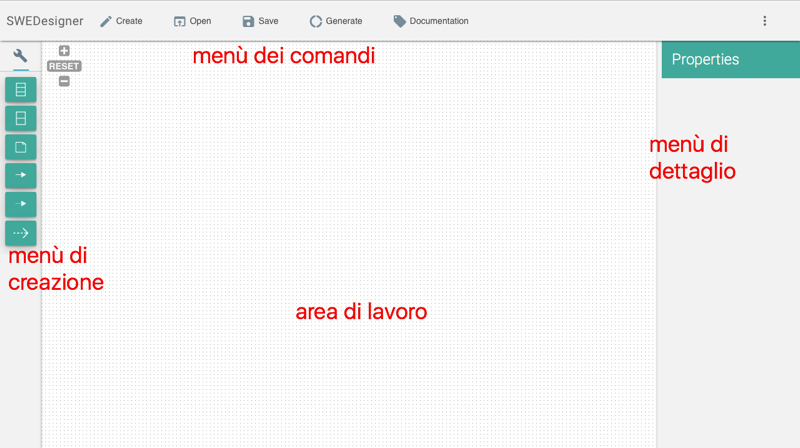
\includegraphics[scale=0.46]{img/index}
	\caption{Interfaccia grafica.}
	\label{fig:screen}
\end{figure}



\subsection{Progettare una nuova applicazione} \label{sec:new}

\subsubsection{Creare un nuovo progetto}
Un diagramma delle classi vuoto rappresenta un nuovo progetto; se vi trovate già davanti a un diagramma vuoto potete iniziare subito a progettare una nuova applicazione, saltando questa sezione e continuando alla sezione \ref{par:arch}. Invece, nel caso abbiate un diagramma delle classi non vuoto ma vogliate creare un nuovo progetto da zero, cliccate sull'icona del menù in alto a sinistra; dal menù a comparsa, cliccate su \click{New Project}; vi ritroverete con un diagramma delle classi vuoto, corrispondente ad un nuovo progetto.

\subsubsection{Progettare l'architettura dell'applicazione} \label{par:arch}
Progettare un'applicazione ad oggetti vuol dire innanzitutto specificarne l'architettura. Per fare ciò, dovete popolare il diagramma (nell'area di lavoro) con delle componenti, che possono essere classi o interfacce.

\paragraph{Creazione di una componente} \label{par:creaz_class} Potete creare una nuova componente cliccando su un'icona del menù di creazione (visibile a sinistra) e cliccando nel punto dell'area di lavoro in cui volete che si materializzi la componente; ci sono tre icone che rappresentano tre tipi di componente dell'architettura:
\begin{itemize}
	\item \click{Class} (1, in figura \ref{fig:creation_class});
	\item \click{Abstract Class} (2, in figura \ref{fig:creation_class});
	\item \click{Interface} (3, in figura \ref{fig:creation_class}).
\end{itemize}
Oltre a queste, altre icone permettono la creazione di commenti (l'icona \click{Comment}; 4, in figura \ref{fig:creation_class}) e di relazioni tra componenti (\click{Generalization}, \click{Implementation} e \click{Association}, che verranno introdotte tra poco; risp. 5, 6 e 7 in figura \ref{fig:creation_class}).

% screenshot menù di creazione
\begin{figure}[h]
\centering
	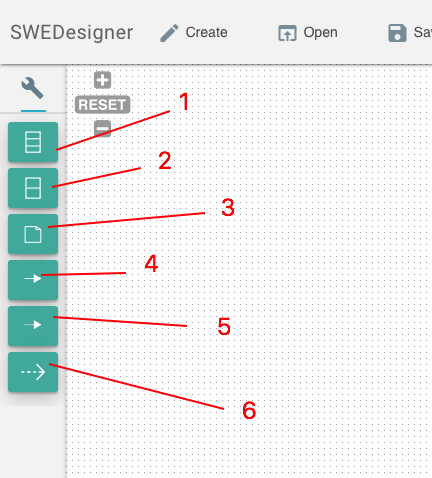
\includegraphics[scale=0.4]{img/creation_class}
	\caption{Il menù di creazione del diagramma delle classi.}
	\label{fig:creation_class}
\end{figure}

\paragraph{Specifica dell'interfaccia di una componente} \label{par:inter} Ogni componente è rappresentata nel diagramma da un rettangolo con due o tre aree, come da standard UML:
\begin{enumerate}
	\item l'area superiore reca il nome della componente;
	\item l'area a metà contiene i campi dati (non presente nelle interfacce);
	\item l'area inferiore contiene i metodi.
\end{enumerate}

Inizialmente le aree contenente campi dati e metodi sono vuote. Per inserire un campo dati in una classe, cliccate sulla classe; dopodiché:
\begin{enumerate}
	\item il menù di dettaglio (a destra) si riempirà con i dettagli della classe cliccata;
	\item cliccate su \click{Attributes} per far comparire l'elenco dei campi dati (attributi);
	\item vi verrà presentato l'elenco dei campi dati;
	\item scorrete in basso e cliccate su \click{Add attribute};
	\item compilate la form per creare il nuovo campo dati.
\end{enumerate}

Per aggiungere un metodo ad una componente del progetto, cliccate sulla classe o sull'interfaccia; dopodiché:
\begin{enumerate}
	\item il menù di dettaglio (a destra) si riempirà con i dettagli della classe cliccata;
	\item cliccate su \click{Methods} per far comparire l'elenco dei metodi;
	\item vi verrà presentato l'elenco dei metodi;
	\item scorrete in basso e cliccate su \click{Add method};
	\item compilate la form per specificare la segnatura del nuovo metodo.
\end{enumerate}
Dopo aver specificato la segnatura di un metodo, bisognerà stabilirne anche il comportamento; per modificare il comportamento di un metodo, si veda §\ref{sec:activity}.

\paragraph{Definizione di una relazione tra due componenti} È possibile definire una relazione tra due componenti del diagramma delle classi. Per fare questo, cercate il tipo di relazione desiderato nel menù di creazione (a sinistra) e cliccate sopra all'icona appropriata; cliccate ora una componente $A$ e poi una componente $B$: questo farà comparire una freccia da $A$ a $B$. Potete, inoltre, trascinare ognuna delle due punte su una nuova componente, cambiando così i membri della relazione. Vi sono tre tipi di relazione:
\begin{itemize}
	\item \click{Generalization}, per estendere l'interfaccia di una classe;
	\item \click{Implementation}, per implementare un'interfaccia pura;
	\item \click{Association}, per suggerire che una componente dipende da un'altra. % TODO
\end{itemize}

% screenshot esempio relazione tra componenti
\begin{figure}[h]
\centering
	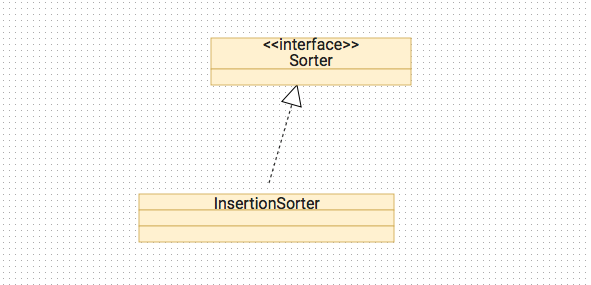
\includegraphics[scale=0.4]{img/relationship}
	\caption{Esempio di relazione tra due componenti: implementazione di \texttt{Sorter} da parte di \texttt{InsertionSorter}.}
	\label{fig:relationship}
\end{figure}

\paragraph{Modificare campi dati e metodi} Per modificare un campo dati o un metodo di una componente, cliccate su di essa; dopodiché:
\begin{enumerate}
	\item il menù di dettaglio (a destra) si riempirà con i dettagli della componente;
	\item cliccate su \click{Attributes} (per far comparire l'elenco dei campi dati) o su \click{Methods} (per far comparire l'elenco dei metodi);
	\item vi verrà presentato l'elenco dei campi dati o dei metodi, a seconda di ciò che avete cliccato;
	\item cercate il campo dati o metodo che volete modificare;
	\item modificate la form contenente i dettagli del campo dati o metodo.
\end{enumerate}


\subsubsection{Definire il comportamento delle componenti} \label{sec:activity}
Mentre la segnatura dei metodi di una componente definisce l'interfaccia di questa, l'implementazione dei metodi definisce il \textbf{comportamento} della componente. Quando avete chiaro quale dev'essere il comportamento di una vostra componente, cercate la componente nel diagramma delle classi e cliccate su di essa; dopodiché:
\begin{enumerate}
	\item il menù di dettaglio (a destra) si riempirà con i dettagli della componente;
	\item cliccate su \click{Methods} per far comparire l'elenco dei metodi;
	\item compilate la form con la segnatura del metodo;
	\item in basso, cliccate su \click{Go to Activity Diagram}.
\end{enumerate}
Al posto del diagramma delle classi, comparirà il \textbf{diagramma di attività} del metodo selezionato.

% screenshot menù di creazione
\begin{figure}[h]
\centering
	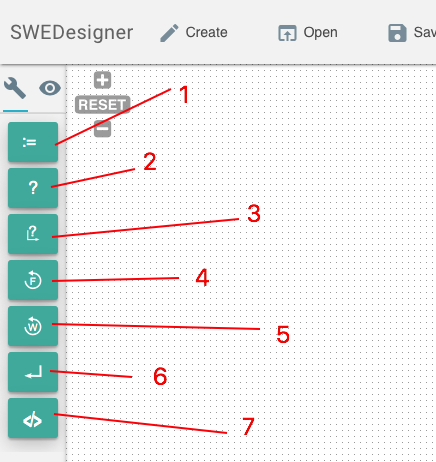
\includegraphics[scale=0.4]{img/creation_activity}
	\caption{Il menù di creazione del diagramma di attività.}
	\label{fig:creation_activity}
\end{figure}

\paragraph{Creazione di blocchi} Ogni metodo è un algoritmo e, in quanto tale, per implementarlo dovete specificare la sequenza di passi che il metodo deve seguire. Ogni passo del metodo può essere una singola istruzione (come un'assegnazione) oppure un'istruzione composita (come un ciclo o un blocco condizionale). Ogni istruzione --- singola o composita --- è rappresentata da un \textbf{blocco} con un riquadro colorato; la barra di creazione (a sinistra) offre diversi tipi di blocchi:
\begin{itemize}
	\item \click{Variable} (1, in figura \ref{fig:creation_activity}) dichiara e/o inizializza una nuova variabile, oppure esegue un'operazione su una variabile (assegnazione o chiamata di metodo); è riconoscibile dal riquadro color giallo ocra.
	\item \click{If} (2, in figura \ref{fig:creation_activity}) esegue una sequenza di blocchi solo se vale una condizione; è riconoscibile dal riquadro color verde smeraldo.
	\item \click{Else} (3, in figura \ref{fig:creation_activity}) esegue una sequenza di blocchi solo se non vale la condizione di un blocco \click{If} immediatamente precedente; è riconoscibile dal riquadro color verde scuro.
	\item \click{For} (4, in figura \ref{fig:creation_activity}) esegue ciclicamente una sequenza di blocchi (ogni iterazione del ciclo è parametrizzata su una variabile); è riconoscibile dal riquadro color rosso.
	\item \click{While} (5, in figura \ref{fig:creation_activity}) esegue ciclicamente una sequenza di blocchi finché vale una condizione; è riconoscibile dal riquadro color blu.
	\item \click{Return} (6, in figura \ref{fig:creation_activity}) esce dal metodo e ritorna il valore specificato; è riconoscibile dal riquadro color arancione.
	\item \click{Custom} (7, in figura \ref{fig:creation_activity}) permette di inserire manualmente del codice che verrà copiato direttamente nel codice sorgente; è riconoscibile dal riquadro color viola.
\end{itemize}
Cliccando su uno dei blocchi nella barra di creazione, esso verrà inserito nella sequenza di passi del metodo. Ogni nuovo blocco su cui cliccherete verrà inserito in coda ai blocchi precedentemente inseriti. In figura \ref{fig:algorithm} potete vedere un semplice esempio di come verrà il diagramma di attività di un metodo.

% screenshot esempio di algoritmo
\begin{figure}[h]
\centering
	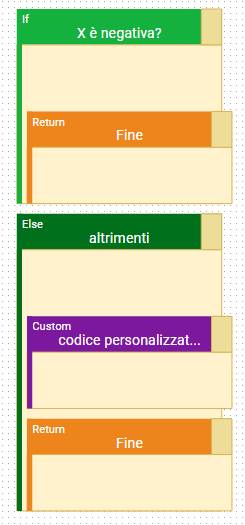
\includegraphics[scale=0.4]{img/algorithm}
	\caption{Esempio di diagramma di attività di un metodo.}
	\label{fig:algorithm}
\end{figure}

\paragraph{Spostamento di blocchi} Ovviamente potete spostare ogni blocco creato e posizionarlo dove volete nella sequenza di passi. Inoltre, potete decidere di inserire un blocco (di qualsiasi tipo) all'interno di un \click{For}, di un \click{While}, di un \click{If} o di un \click{Else}: questi tre tipi di blocchi possono contenerne altri. Per rimarcare che un blocco sta all'interno di un altro, esso viene “indentato”, cioè spostato leggermente a destra rispetto al blocco che lo contiene.

\paragraph{Rimozione di blocchi} Per rimuovere un blocco da un diagramma di attività, passate sul blocco con il mouse: comparirà una “X” su sfondo rosso che potrete cliccare per rimuovere il blocco.

\subsubsection{Modificare l'architettura}
Una volta modificata l'implementazione di un metodo, per modificare l'architettura dell'intera applicazione dovete tornare al diagramma delle classi. Per fare ciò, cliccate sul pulsante in basso a destra \click{Back to Class Diagram}. Il diagramma di attività modificato verrà salvato e, al suo posto, vi verrà presentato il diagramma delle classi.

Dal diagramma delle classi, potete modificare l'architettura dell'applicazione in vari modi: potete spostare o rimuovere ogni relazione tra componenti dell'applicazione e potete aggiungere o rimuovere componenti. Per aggiungere una componente, tornate alla sezione \ref{par:creaz_class}; per rimuoverla, passateci sopra con il mouse: comparirà una “X” su sfondo rosso che potrete cliccare per rimuovere la componente.



\subsection{Salvare il progetto} \label{sec:save}

Ad ogni momento, è possibile salvare i diagrammi disegnati nel proprio computer. Per salvare un progetto (cioè un insieme di diagrammi), navigate il menù dei comandi (in alto) e cliccate \click{Save}. Verrà avviato il download di un singolo file JSON: questo file (con estensione \texttt{.json}) rappresenta il vostro progetto e contiene tutte le informazioni sui diagrammi che avete disegnato.



\subsection{Caricare un progetto} \label{sec:load}

Se volete lavorare ad un progetto che avete precedentemente salvato, navigate il menù dei comandi e cliccate \click{Load}. Il vostro browser vi chiederà di indicare quale file volete caricare: scegliete il file JSON che desiderate e cliccate \click{Ok}. \proj{} verrà popolato con i dati del file JSON caricato. Potete ora continuare a lavorare sul progetto che avevate salvato e, in seguito, salvarlo di nuovo.



\subsection{Generare un eseguibile dal progetto} \label{sec:gen}

Quando, infine, i diagrammi che avrete disegnato vi sembreranno sufficienti, potrete generare da essi un programma eseguibile. Per fare questo, navigate il menù dei comandi e cliccate \click{Generate}. Il vostro browser invierà una richiesta di generazione al nostro server. La risposta del server può essere positiva (vi viene inviato il codice eseguibile, assieme al codice sorgente) o negativa. Quest'ultimo caso si può verificare per vari motivi; il più probabile è che non abbiate progettato bene la vostra applicazione. Se è così, pensate a modificare i vostri diagrammi e riprovate. Si veda §\ref{sec:mal_gen} per gestire bene una risposta negativa del server.



\subsection{Funzionalità accessorie} \label{sec:extra}

Di seguito presentiamo le funzionalità secondarie di \proj{} e come sia possibile utilizzarle.

\subsubsection{\emph{Pan \& Zoom} (ingrandimento e riduzione)}
È possibile ingrandire e rimpicciolire l'area di lavoro. Per farlo, è sufficiente muovere la rotellina del mouse in alto o in basso. È possibile anche muovere l'area di lavoro premendo in una zona vuota, muovendo e rilasciando il mouse. 

In alternativa alla rotella del mouse, potete usare i pulsanti presenti in alto a destra, \click{+}, \click{-} e \click{RESET}, rispettivamente al fine di ingrandire, ridurre e reimpostare il livello di zoom.

\subsubsection{Visualizzazione estesa e compatta}
Al fine di aumentare l'area di disegno disponibile, le barre laterali occupano il minor spazio possibile (“visualizzazione compatta”). Esiste, tuttavia, la possibilità di avere le barre laterali più spaziose (“visualizzazione estesa”, come in figura \ref{fig:extended}); per fare questo è sufficiente premere sul menù in alto a destra in corrispondenza dei tre punti verticali (vedi sempre figura \ref{fig:extended}) e selezionare \click{Extended}. Per tornare alla visualizzazione compatta, basta tornare al menù in alto a destra e premere \click{Compact}.

% screenshot visualizzazione estesa
\begin{figure}[h]
\centering
	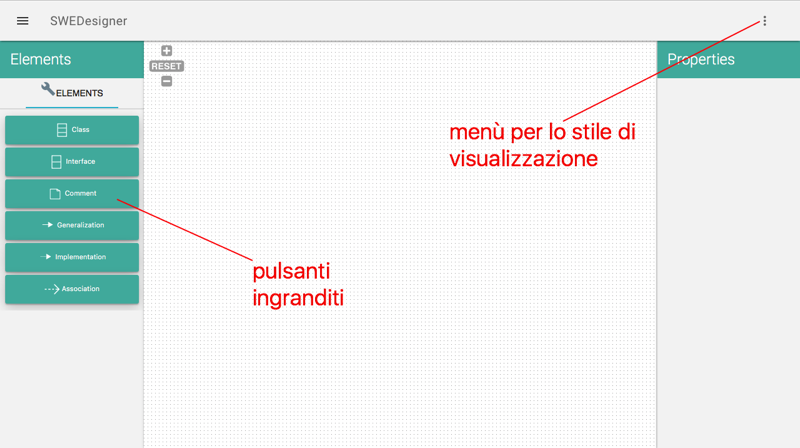
\includegraphics[scale=0.4]{img/extended}
	\caption{Visualizzazione “estesa” di \proj.}
	\label{fig:extended}
\end{figure}

\subsubsection{\emph{Treeview}}
All'interno del diagramma delle attività è possibile far comparire, al posto del menù di creazione, un albero (detto \emph{Treeview}) contenente tutte le classi e i loro attributi.

I simboli da cui i nomi sono preceduti indicano ciò che i vari elementi rappresentano. Questa è l'associazione tra elemento e simbolo grafico:
\begin{itemize}
	\item \textbf{classe}: tre elementi di colore differente;
	\item \textbf{metodo}: rombo viola;
	\item \textbf{interfaccia}: chiave blu;
	\item \textbf{attributo}: tondo blu.
\end{itemize}

Sfruttiamo la medesima simbologia per la funzione di autocompletamento (vedi §\ref{sec:autocomplete}).

\subsubsection{Autocompletamento} \label{sec:autocomplete}
Mentre riempite il contenuto di un blocco del diagramma di attività, potete sfruttare la funzionalità di autocompletamento. Per usarla, è sufficiente cominciare a scrivere la variabile desiderata: automaticamente, \proj{} vi fornirà i suggerimenti più appropriati per completare il testo inserito.



%%%%%%%%%%%%%%%%%%%%%%%%%%%%
%%  Risoluzione dei problemi
%%%%%%%%%%%%%%%%%%%%%%%%%%%%

\section{Risoluzione dei problemi} \label{sec:problemi}

È possibile riscontrare dei problemi nei seguenti ambiti:
\begin{enumerate}
	\item durante l'esecuzione del programma generato;
	\item nel tentativo di accedere all'applicazione;
	\item nell'utilizzo dell'applicazione stessa.
\end{enumerate}



\subsection{Programma generato malfunzionante} \label{sec:mal_gen}

Può capitare che l'applicazione generata, mente la eseguite, si interrompa bruscamente a causa di un'eccezione o per qualche altro motivo. In questi casi la causa va ricercata principalmente nella progettazione dell'applicazione, cioè nel momento in cui voi avete disegnato i diagrammi dell'applicazione.

In particolare, possibili cause di malfunzionamento della vostra applicazione posso essere (dalla più probabile alla meno probabile):
\begin{itemize}
	\item avete omesso di gestire qualche eccezione;
	\item avete previsto un metodo ricorsivo che sopravvaluta la memoria della vostra macchina;
	\item avete inserito un “blocco custom” maligno nel diagramma di qualche metodo, cioè un'istruzione legittima che però interrompe la vostra applicazione;
	\item avete altrimenti introdotto qualche bug non segnalato in progettazione né in compilazione;
	\item avete trovato un bug in \proj.
\end{itemize}



\subsection{Accesso all'applicazione non possibile}

Nel caso non riusciate ad accedere al nostro server, potete recarvi all'indirizzo \url{http://www.downforeveryoneorjustme.com} per verificare se il problema è relativo al vostro provider o al nostro server.



\subsection{Problemi con l'utilizzo di \proj}

È possibile che \proj{} contenga dei piccoli bug, oppure che sia desiderabile una modifica del suo funzionamento. Potete segnalare qualsiasi malfunzionamento o richiesta di funzionalità all'indirizzo \url{https://github.com/hivex-unipd/swedesigner/issues}, sotto forma di \emph{GitHub Issue}.





\appendix

%%%%%%%%%%%%%%%%%%%%%%%%%%%%%%%
%%  Glossario dei termini utili
%%%%%%%%%%%%%%%%%%%%%%%%%%%%%%%

\section{Glossario dei termini utili} \label{app:gloss}

\begin{description}
	\item[algoritmo] Sequenza\marginpar{\textbf{A}} di passi per raggiungere un obiettivo.
	\item[applicazione web] Applicazione accessibile via browser.
	\item[attributo] In programmazione a oggetti, variabile che deve appartenere ad ogni istanza di una classe.
	\item[assegnazione] In programmazione, istruzione che imposta una variabile a un determinato valore.
	\item[blocco] In\marginpar{\textbf{B}} un diagramma di attività \proj, rettangolo corrispondente al passo di una procedura, cioè a un'istruzione; un blocco \click{For}, \click{While}, \click{If} o \click{Else} può contenere altri blocchi.
	\item[campo dati] Vedi\marginpar{\textbf{C}} “attributo”.
	\item[ciclo] In programmazione, istruzione che specifica una condizione logica e una sequenza di istruzioni da eseguire ripetutamente finché vale la condizione logica. In \proj, un ciclo è un blocco \click{For} o \click{While}.
	\item[classe] In programmazione a oggetti, categoria di oggetti che presentano la medesima interfaccia e il medesimo comportamento.
	\item[diagramma delle classi] Diagramma\marginpar{\textbf{D}} UML che descrive l'architettura di un sistema orientato agli oggetti, mostrando le classi, le loro proprietà, il loro comportamento e le loro relazioni.
	\item[diagramma di attività] In \proj, diagramma che specifica i passi di una procedura rappresentando ogni passo come un blocco rettangolare (vedi “blocco”).
	\item[estensione] In\marginpar{\textbf{E}} programmazione a oggetti, relazione tra due classi in cui una classe garantisce di offrire un sovrainsieme dell'interfaccia (vedi “interfaccia --- 1”) della classe estesa.
	\item[indentazione] Nel\marginpar{\textbf{I}} codice sorgente di un programma, differenza tra la distanza di una riga di codice rispetto al margine sinistro e la distanza (rispetto allo stesso margine) dell'istruzione composita contenente tale riga di codice.
	\item[interfaccia] In programmazione a oggetti, (1) l'insieme di servizi offerti da una classe oppure (2) una classe che specifica la segnatura dei suoi metodi ma non la loro implementazione.
	\item[istruzione condizionale] In programmazione, istruzione che specifica una condizione logica e una sequenza di istruzioni da eseguire solo se vale la condizione logica. In \proj, un'istruzione condizionale è un blocco \click{If} (eventualmente seguito da un blocco \click{Else}).
	\item[metodo] In\marginpar{\textbf{M}} programmazione a oggetti, servizio (procedura) offerto da ogni oggetto appartenente ad una certa classe.
	\item[oggetto] In\marginpar{\textbf{O}} programmazione, variabile appartenente ad una classe (vedi “variabile”).
	\item[UML] Unified\marginpar{\textbf{U}} Modelling Language: famiglia di notazioni grafiche che si basano su un singolo meta-modello e servono a descrivere e progettare sistemi software.
	\item[variabile] In\marginpar{\textbf{V}} programmazione, entità che ha un valore e una locazione in memoria.
\end{description}



\end{document}
